\chapter{क्रोमैटिन और एपिजेनेटिकी}\label{ch:b3:chromatin-epigenetics}

एक ही प्रसव के दो चूहे, अंतिम क्षार तक आनुवंशिक रूप से समरूप, अगल-बगल
बैठे हैं: एक दुबला और भूरा है, दूसरा मोटा और पीला, और वही मधुमेही
होगा। कोई कैलिको बिल्ली नारंगी और काले धब्बे पहने रहती है, यद्यपि उसकी
त्वचा की हर कोशिका में वही दो X गुणसूत्र हैं। किसी बच्चे को गुणसूत्र 15
का वही विलोपित खंड मिलता है जो किसी दूसरे बच्चे को मिला है, और एक को
प्रैडर--विली संलक्षण होता है तो दूसरे को एंजेलमैन संलक्षण --- अंतर केवल
इतना है कि विलोपन किस जनक से आया। इसमें से कुछ भी DNA अनुक्रम में लिखा
नहीं है। वह उसके \emph{ऊपर} लिखा है: इसमें कि दो मीटर DNA दस
माइक्रोमीटर चौड़े केंद्रक में किस तरह ठूँसा जाता है, उन छोटे रासायनिक
समूहों में जो संवेष्टक प्रोटीनों से और स्वयं साइटोसीनों से जुड़े हैं,
और उस तंत्र में जो उन चिह्नों की नकल एक कोशिका से उसकी पुत्रियों तक
पहुँचाता है। यह अध्याय सूचना की उसी दूसरी परत के बारे में है, उसके
आणविक वाहकों के बारे में, और इस बारे में कि वह ईमानदारी से कितना याद
रख सकती है।

\section{क्रोमैटिन: तकले पर लिपटा DNA}

\begin{definition}[न्यूक्लियोसोम और क्रोमैटिन]\label{def:b3:chromatin-epigenetics:nucleosome}
\index{न्यूक्लियोसोम}\index{क्रोमैटिन}\index{हिस्टोन}\index{सुक्रोमैटिन}\index{विषमक्रोमैटिन}
\emph{क्रोमैटिन} DNA का प्रोटीनों के साथ बना वह संकुल है जिसके रूप में
सुकेंद्रकी केंद्रक में जीनोम रहता है। उसकी पुनरावर्ती इकाई
\emph{न्यूक्लियोसोम} है: \qty{147}{bp} DNA, जो किसी \emph{हिस्टोन}
अष्टलक --- छोटे, अत्यंत क्षारीय प्रोटीनों H2A, H2B, H3 और H4 की दो-दो
प्रतियों --- के चारों ओर $1.65$ वामावर्त फेरों में लिपटा है, और उसके
बाद अगले न्यूक्लियोसोम तक \qtyrange{20}{60}{bp} का एक \emph{योजक}।
पाँचवाँ हिस्टोन H1 योजक से वहाँ बँधता है जहाँ वह क्रोड में घुसता और
उससे निकलता है, और मनकों को एक-दूसरे से सटाकर जमने में मदद करता है। हर
क्रोड-हिस्टोन पर लगभग \numrange{20}{40} अवशेषों की एक असंरचित
अमीनो-सिरे वाली \emph{पूँछ} होती है, जो कण से बाहर निकली रहती है। जो
क्रोमैटिन हल्का अभिरंजित होता है, ढीला बँधा है और अनुलेखित होता है, वह
\emph{सुक्रोमैटिन} है; सघन बँधा, देर से प्रतिकृत होने वाला और प्रायः
मौन क्रोमैटिन, जो गुणसूत्रबिंदुओं, टीलोमियरों और पुनरावर्ती अनुक्रमों
पर मिलता है, \emph{विषमक्रोमैटिन} है।
\end{definition}

\begin{proof}[प्रमाण-सामग्री]
ह्यूइश और बर्गोइन (1973) ने चूहे के यकृत-केंद्रकों को एक अंतर्जात
न्यूक्लिएज़ से पचाया और पाया कि DNA धब्बे के रूप में नहीं, बल्कि ऐसे
खंडों की सीढ़ी के रूप में निकला जिनकी लंबाइयाँ लगभग \qty{200}{bp} की
गुणज थीं: DNA नियमित अंतरालों पर सुरक्षित था और केवल उनके बीच कटा।
कॉर्नबर्ग (1974) ने दिखाया कि सुरक्षित इकाई आठ \omterm{def:b3:chromatin-epigenetics:nucleosome}{हिस्टोनों} का ऐसा कण है
जिसके साथ लगभग \qty{200}{bp} है, और धीरे से फैलाए गए \omterm{def:b3:chromatin-epigenetics:nucleosome}{क्रोमैटिन} के
इलेक्ट्रॉन सूक्ष्मचित्रों में ``डोरी पर मनके'' दिखाई दिए। लूगर और
सहयोगियों (1997) ने क्रोड-कण की क्रिस्टल संरचना \qty{2.8}{\angstrom}
पर हल की: \qty{147}{bp}, एक अष्टलक जिसकी पूँछें DNA की कुंडलियों के
बीच से बाहर निकलती हैं।
\end{proof}

\begin{omfigure}
\begin{tikzpicture}[every node/.style={font=\scriptsize}, >=stealth]
  % beads on a string
  \foreach \x/\y in {0/0, 2.2/0.5, 4.4/0, 6.6/0.5, 8.8/0} {
    \fill[omDef!30] (\x,\y) circle (0.42);
    \draw[very thick, omThm!70!black] (\x,\y) circle (0.5);
  }
  \draw[very thick, omThm!70!black] (-1.1,-0.1) -- (0-0.47,-0.17);
  \draw[very thick, omThm!70!black] (0.47,-0.17) -- (2.2-0.47,0.33);
  \draw[very thick, omThm!70!black] (2.67,0.33) -- (4.4-0.47,-0.17);
  \draw[very thick, omThm!70!black] (4.87,-0.17) -- (6.6-0.47,0.33);
  \draw[very thick, omThm!70!black] (7.07,0.33) -- (8.8-0.47,-0.17);
  \draw[very thick, omThm!70!black] (9.27,-0.17) -- (10.4,-0.1);
  % tails
  \foreach \x/\y in {0/0, 4.4/0, 8.8/0} { \draw[omProp, thick] (\x,\y+0.5) .. controls (\x-0.2,\y+0.9) .. (\x+0.1,\y+1.15); \draw[omProp, thick] (\x,\y-0.5) .. controls (\x+0.2,\y-0.9) .. (\x-0.1,\y-1.15); }
  \foreach \x/\y in {2.2/0.5, 6.6/0.5} { \draw[omProp, thick] (\x,\y+0.5) .. controls (\x-0.2,\y+0.9) .. (\x+0.1,\y+1.15); }
  % H1
  \fill[omMeth!70!black] (1.55,0.05) circle (0.12); \fill[omMeth!70!black] (5.95,0.05) circle (0.12);
  % labels
  \node[above, align=center] at (2.2,1.75) {हिस्टोन पूँछें\\(ऐसीटिलीकरण, मेथिलीकरण)};
  \node[below, align=center] at (4.4,-1.35) {क्रोड-कण: अष्टलक\\$+$ \qty{147}{bp}, $1.65$ फेरे};
  \node[below, align=center] at (7.7,-0.55) {योजक DNA\\\qtyrange{20}{60}{bp}};
  \node[below] at (5.95,-0.1) {H1};
  \draw[<->] (-0.5,-2.2) -- (2.2-0.5,-2.2) node[midway, below] {पुनरावृत्ति $\approx \qty{200}{bp}$, \qty{11}{nm}};
  \draw[gray] (-0.5,-1.95) -- (-0.5,-2.35); \draw[gray] (1.7,-1.95) -- (1.7,-2.35);
\end{tikzpicture}

{\small \qty{10}{nm} तंतु: सतत DNA (लाल) पर \omterm{def:b3:chromatin-epigenetics:nucleosome}{न्यूक्लियोसोम} क्रोड (नीले),
हर मनका अपनी पूँछें (नारंगी) बाहर निकाले एक \omterm{def:b3:chromatin-epigenetics:nucleosome}{हिस्टोन} अष्टलक, और
प्रवेश--निकास बिंदु पर योजक \omterm{def:b3:chromatin-epigenetics:nucleosome}{हिस्टोन} H1 (हरा)। लगभग छह \omterm{def:b3:chromatin-epigenetics:nucleosome}{न्यूक्लियोसोम}
उतनी लंबाई घेरते हैं जितनी नग्न DNA के \qty{1200}{bp} घेरते।}
\end{omfigure}

\begin{omfigure}
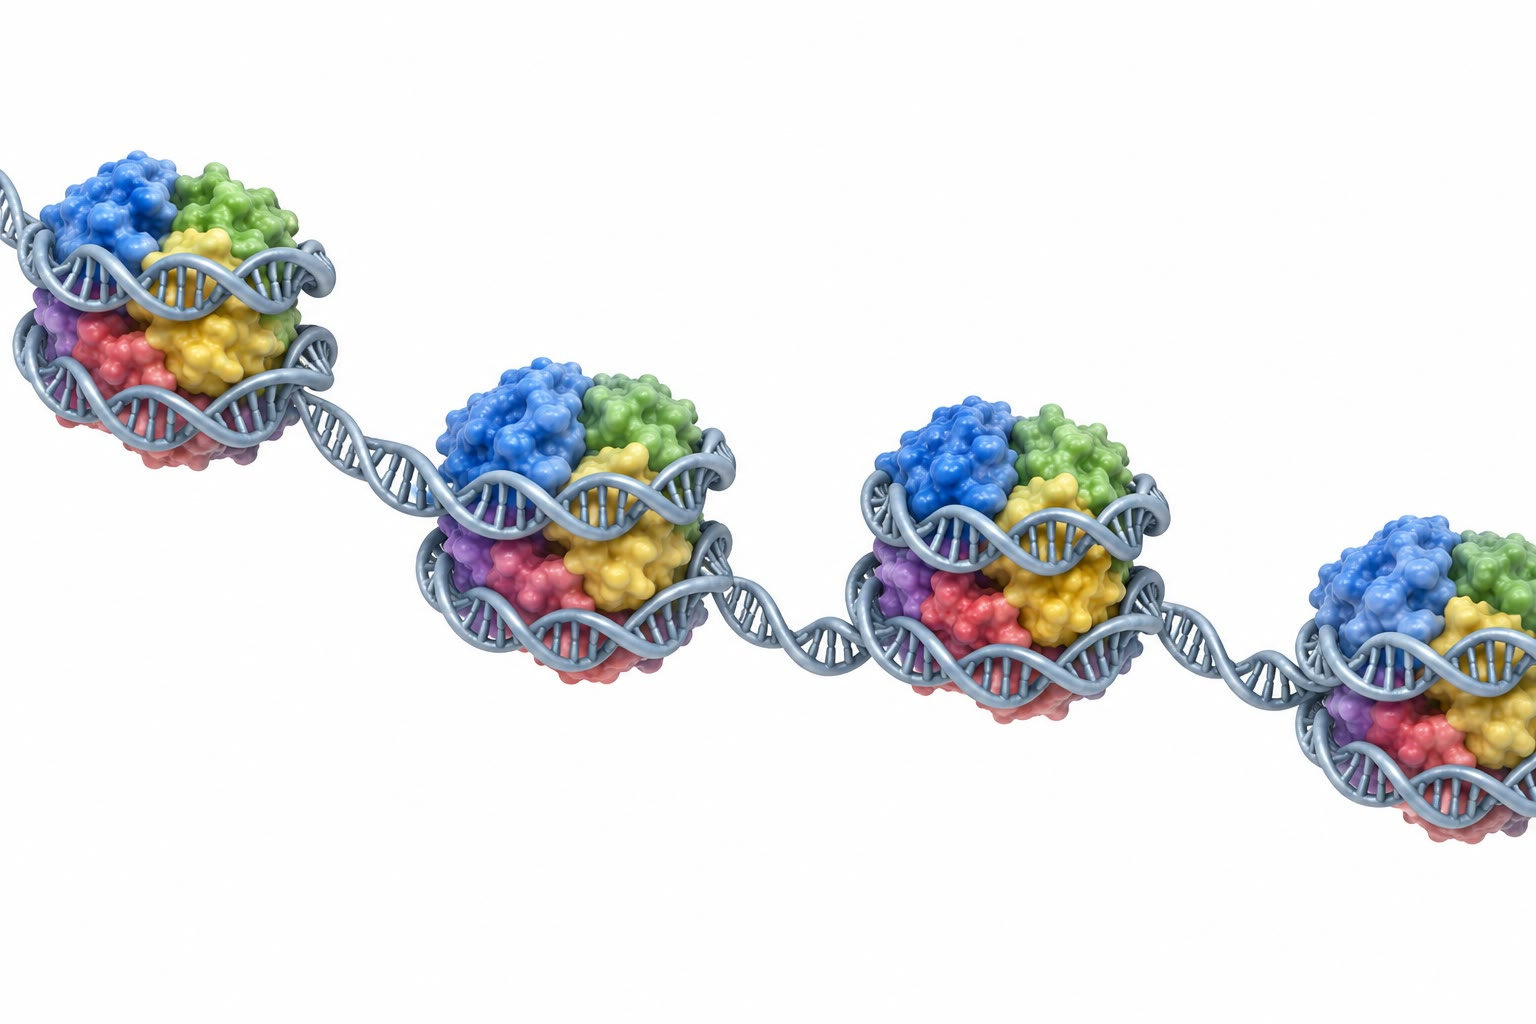
\includegraphics[width=0.6\linewidth]{images/book5/ai/b5-01-nucleosomes.jpg}

{\small आणविक पैमाने पर \omterm{def:b3:chromatin-epigenetics:nucleosome}{क्रोमैटिन}: क्रमिक \omterm{def:b3:chromatin-epigenetics:nucleosome}{हिस्टोन} क्रोडों के चारों ओर
लिपटी दोहरी कुंडली, वही ``डोरी पर मनके'' जिन्हें न्यूक्लिएज़ की सीढ़ी
ने उजागर किया।}
\end{omfigure}

\begin{proposition}[संघनन के स्तर]\label{prop:b3:chromatin-epigenetics:compaction}
\index{संवेष्टन अनुपात}\index{क्रोमैटिन पाश}\index{सांस्थितिक सहचारी प्रांत}
किसी \omterm{def:b3:chromatin-epigenetics:nucleosome}{क्रोमैटिन} संरचना का \emph{\omterm{prop:b3:chromatin-epigenetics:compaction}{संवेष्टन अनुपात}} उसमें निहित DNA की
लंबाई को उस संरचना की लंबाई से भाग देने पर मिलता है। \qty{10}{nm}
तंतु में लिपटने से लगभग $6$ का अनुपात बनता है: \qty{200}{bp} की
पुनरावृत्ति के \qty{68}{nm} एक ही \qty{11}{nm} मनके में सिमट जाते हैं।
अंतरावस्था केंद्रक में तंतु किसी नियमित मोटे तंतु में नहीं लिपटता,
जैसा पाठ्यपुस्तकें बहुत समय तक बनाती रहीं, बल्कि दसियों से सैकड़ों
किलोक्षार के \emph{पाशों} में मुड़ता है, जिन्हें उनके आधारों पर
वलयाकार कोहेसिन संकुल और DNA-बंधक प्रोटीन CTCF थामे रहते हैं; ये पाश
लगभग एक मेगाक्षार के \emph{\omterm{prop:b3:chromatin-epigenetics:compaction}{सांस्थितिक सहचारी प्रांत}} (TAD) बनाते हैं,
जिनके भीतर कोई जीन अपने नियामकों से बाहर की किसी भी चीज़ की तुलना में
कहीं अधिक बार मिलता है। समसूत्री गुणसूत्र, सबसे संघनित अवस्था, का
\omterm{prop:b3:chromatin-epigenetics:compaction}{संवेष्टन अनुपात} \num{10000} के निकट है: किसी औसत मानव गुणसूत्र का
\qty{4}{cm} DNA \qty{4}{\micro m} लंबी छड़ में मुड़ा रहता है।
\end{proposition}

\begin{example}[दस माइक्रोमीटर में दो मीटर]\label{ex:b3:chromatin-epigenetics:two-metres}
किसी मानव द्विगुणित केंद्रक में $6.4\times 10^{9}$ क्षार युग्म हैं।
प्रति क्षार युग्म \qty{0.34}{nm} की दर से यह \qty{2.2}{m} दोहरी कुंडली
है, और केंद्रक लगभग \qty{10}{\micro m} चौड़ा है। वह
$6.4\times 10^{9}/200 \approx 3.2\times 10^{7}$ \omterm{def:b3:chromatin-epigenetics:nucleosome}{न्यूक्लियोसोमों} में
ठुँसी है, जिनमें से हर एक पर DNA के \qty{96}{kDa} के सामने लगभग
\qty{108}{kDa} \omterm{def:b3:chromatin-epigenetics:nucleosome}{हिस्टोन} है (\qty{650}{Da} प्रति युग्म की दर से
\qty{147}{bp}): द्रव्यमान की दृष्टि से केंद्रक में लगभग उतना ही
\omterm{def:b3:chromatin-epigenetics:nucleosome}{हिस्टोन} है जितना DNA। स्वयं DNA को \qty{2}{nm} चौड़ा बेलन मानें तो
उसका आयतन केवल लगभग \qty{7}{\micro m^3} है, यानी \qty{5}{\micro m}
त्रिज्या के गोलाकार केंद्रक का लगभग \qty{1}{\%}; संवेष्टन की समस्या
उलझाव और पहुँच की है, जगह की नहीं।
\end{example}

\section{हिस्टोन कूट}

\begin{definition}[हिस्टोन रूपांतरण]\label{def:b3:chromatin-epigenetics:histone-code}
\index{हिस्टोन कूट}\index{ऐसीटिलीकरण}\index{हिस्टोन मेथिलीकरण}\index{लेखक}\index{पाठक}\index{विलोपक}
\omterm{def:b3:chromatin-epigenetics:nucleosome}{हिस्टोन} पूँछों के अवशेष सहसंयोजी रूप से रूपांतरित होते हैं: लाइसीनों का
\emph{ऐसीटिलीकरण} (जो उनका धन आवेश उदासीन कर देता है और DNA पर पकड़
ढीली कर देता है), लाइसीनों और आर्जिनीनों का \emph{मेथिलीकरण} (एक, दो
या तीन मेथिल समूह, आवेश में बिना किसी बदलाव के), सेरीनों का
फ़ॉस्फ़ोरिलीकरण, लाइसीनों का यूबिक्विटिनीकरण। किसी रूपांतरण का नाम
\omterm{def:b3:chromatin-epigenetics:nucleosome}{हिस्टोन}, अवशेष और समूह से बनता है: H3K4me3 यानी \omterm{def:b3:chromatin-epigenetics:nucleosome}{हिस्टोन} H3, लाइसीन 4,
त्रिमेथिलित; H3K27ac यानी H3 की लाइसीन 27 ऐसीटिलित। \emph{\omterm{def:b3:chromatin-epigenetics:nucleosome}{हिस्टोन} कूट}
चिह्नों के संयोजनों और उनके नीचे पड़े जीन की अवस्था के बीच का सहसंबंध
है: सक्रिय प्रवर्तकों और संवर्धकों पर H3K4me3 तथा H3K27ac, अनुलेखित
जीन-पिंडों के साथ-साथ H3K36me3, संघटक \omterm{def:b3:chromatin-epigenetics:nucleosome}{विषमक्रोमैटिन} पर H3K9me3,
परिवर्धन के दौरान मौन किए गए जीनों पर H3K27me3। जो एंज़ाइम कोई चिह्न
जोड़ते हैं वे \emph{लेखक} हैं (\omterm{def:b3:chromatin-epigenetics:nucleosome}{हिस्टोन} ऐसीटिलट्रांसफ़रेज़, HAT;
मेथिलट्रांसफ़रेज़), जो उसे हटाते हैं वे \emph{विलोपक} हैं (\omterm{def:b3:chromatin-epigenetics:nucleosome}{हिस्टोन}
डीऐसीटिलेज़, HDAC; डीमेथिलेज़), और जो प्रोटीन किसी चिह्न से बँधकर उस
पर काम करते हैं वे \emph{पाठक} हैं: कोई \emph{ब्रोमोप्रांत}
ऐसीटिल-लाइसीन से बँधता है, कोई \emph{क्रोमोप्रांत} मेथिल-लाइसीन से।
\end{definition}

\begin{proposition}[चिह्न पढ़े जाते हैं, केवल महसूस नहीं होते]\label{prop:b3:chromatin-epigenetics:readers}
\index{HP1}\index{पॉलीकोम्ब}\index{PRC2}\index{ट्राइथोरैक्स}
\omterm{def:b3:chromatin-epigenetics:histone-code}{ऐसीटिलीकरण} कुछ हद तक स्थिरवैद्युतिकी से काम करता है --- ऐसीटिलित पूँछ
अपने DNA को कम कसकर पकड़ती है और तंतु खुल जाता है --- पर अधिकांश चिह्न
पाठकों को बुलाकर काम करते हैं। H3K9me3 से \emph{\omterm{def:b3:chromatin-epigenetics:nucleosome}{विषमक्रोमैटिन} प्रोटीन
HP1} का क्रोमोप्रांत बँधता है, जो द्विलक बनाता है, पड़ोसी
\omterm{def:b3:chromatin-epigenetics:nucleosome}{न्यूक्लियोसोमों} के बीच सेतु बाँधता है और उसी मेथिलट्रांसफ़रेज़ (SUV39H)
को बुला लेता है जो अगले \omterm{def:b3:chromatin-epigenetics:nucleosome}{न्यूक्लियोसोम} पर H3K9me3 लिखती है: चिह्न तंतु
के साथ-साथ तब तक फैलता है जब तक कोई सीमा न मिले, और जो कुछ वह ढकता है
उसे संघनित कर देता है। H3K27me3 को \emph{पॉलीकोम्ब दमनकारी संकुल 2}
(PRC2, उत्प्रेरक उपइकाई EZH2) लिखता है और PRC1 पढ़ता है, जो H2A का
यूबिक्विटिनीकरण करके तंतु को संघनित करता है, और संकुल स्वयं उसी चिह्न
से उद्दीप्त होता है जो वह बनाता है; प्रोटीनों का \emph{ट्राइथोरैक्स}
समूह विरोधी H3K4me3 लिखता है और किसी दिए हुए कोशिका-प्रकार के
परिवर्धन-जीनों को चालू रखता है। ऐसा हर पाश --- \omterm{def:b3:chromatin-epigenetics:histone-code}{पाठक} \omterm{def:b3:chromatin-epigenetics:histone-code}{लेखक} को बुलाता है
--- वह धन पुनर्भरण है जो किसी अवस्था को एक बार स्थापित हो जाने पर
स्वयं को बनाए रखने देता है, और वंशागत चिह्न को यही चाहिए।
\end{proposition}

\begin{omfigure}
\begin{tikzpicture}[every node/.style={font=\scriptsize}, >=stealth]
  % nucleosomes with tails
  \foreach \x in {0,2,4,6} { \draw[thick, omDef, fill=omDef!20] (\x,0) circle (0.45); \draw[omProp, thick] (\x,0.45) -- (\x,1.15); }
  % marks
  \fill[omThm] (2,1.15) circle (0.11); \fill[omThm] (4,1.15) circle (0.11);
  \fill[omMeth!80!black] (0,1.15) circle (0.11);
  \node[left] at (-0.5,1.15) {ac};
  \node[right, align=left] at (6.15,1.15) {me3};
  % HP1 reader
  \draw[thick, fill=omExo!30] (2.6,1.7) ellipse (0.5 and 0.25); \node at (2.6,1.7) {पाठक};
  \draw[thick, fill=omExo!30] (4.2,2.35) ellipse (0.55 and 0.25); \node at (4.2,2.35) {लेखक};
  \draw[->, thick] (2.9,1.9) -- (3.75,2.2);
  \draw[->, thick, omThm] (4.6,2.15) .. controls (5.6,2.0) and (6.1,1.8) .. (6.05,1.3);
  \node[right, align=left, font=\scriptsize] at (6.6,2.0) {अगले\\न्यूक्लियोसोम तक फैलता है};
  \draw[->, thick, gray] (2.2,1.3) -- (2.45,1.5);
  % eraser
  \draw[thick, fill=omExo!30] (0.6,2.2) ellipse (0.5 and 0.25); \node at (0.6,2.2) {विलोपक};
  \draw[->, thick, omMeth!80!black] (0.3,2.0) -- (0.05,1.35);
  % DNA
  \draw[very thick, omThm!70!black] (-0.9,-0.3) -- (-0.45,-0.05) (0.45,-0.05) -- (1.55,-0.05) (2.45,-0.05) -- (3.55,-0.05) (4.45,-0.05) -- (5.55,-0.05) (6.45,-0.05) -- (7.2,-0.3);
  \node[below, align=center] at (0,-0.6) {खुला: ऐसीटिल समूह\\एक आवेश हटा देता है};
  \node[below, align=center] at (5,-0.6) {बंद: HP1 द्वारा पढ़ा गया H3K9me3,\\जो K9 मेथिलेज़ को बुलाता है};
\end{tikzpicture}

{\small लेखक--पाठक--विलोपक का तर्क। किसी एक \omterm{def:b3:chromatin-epigenetics:nucleosome}{न्यूक्लियोसोम} के चिह्न से
बँधा \omterm{def:b3:chromatin-epigenetics:histone-code}{पाठक} उस \omterm{def:b3:chromatin-epigenetics:histone-code}{लेखक} को बुलाता है जो वही चिह्न अगले पर लगाती है, इसलिए
अवस्था फैलती है और स्वयं की नकल करती है; \omterm{def:b3:chromatin-epigenetics:histone-code}{विलोपक} उसका विरोध करते हैं।
ऐसीटिल समूह (हरे) तंतु खोलते हैं; H3K9me3 (लाल) उसे बंद करता है।}
\end{omfigure}

\begin{method}[क्रोमैटिन प्रतिरक्षा-अवक्षेपण (ChIP)]\label{met:b3:chromatin-epigenetics:chip}
\index{ChIP}\index{क्रोमैटिन प्रतिरक्षा-अवक्षेपण}
यह देखने के लिए कि कोई चिह्न या प्रोटीन जीनोम पर कहाँ बैठा है:
(1) जीवित कोशिकाओं में फ़ॉर्मेल्डिहाइड से प्रोटीनों को DNA से
तिर्यक-बद्ध कीजिए; (2) \omterm{def:b3:chromatin-epigenetics:nucleosome}{क्रोमैटिन} को कुछ सौ क्षार युग्मों के खंडों में
कतर लीजिए; (3) मणिकाओं पर लगे, उस चिह्न (मान लीजिए H3K27me3) के विरुद्ध
प्रतिरक्षी से खंडों को अवक्षेपित कीजिए; (4) तिर्यक-बंध पलटकर DNA शुद्ध
कीजिए; (5) उसका अनुक्रमण कीजिए (ChIP-seq) और जीनोम पर वाचन गिनिए:
शिखर वहीं हैं जहाँ चिह्न था। बिना प्रतिरक्षी वाले निवेश-DNA का एक
नियंत्रण पृष्ठभूमि तय करता है। विभेदन खंडों जितना है, लगभग एक
\omterm{def:b3:chromatin-epigenetics:nucleosome}{न्यूक्लियोसोम}।
\end{method}

\begin{remark}[कूट या सहसंबंध]\label{rem:b3:chromatin-epigenetics:code}
शब्द ``कूट'' बात को बढ़ा-चढ़ाकर कहता है। अनेक चिह्न अनुलेखन के कारण
नहीं, उसके परिणाम हैं (H3K36me3 को पॉलीमरेज़ के साथ चलती एक
मेथिलट्रांसफ़रेज़ जमा करती है), और किसी \omterm{def:b3:chromatin-epigenetics:histone-code}{लेखक} को हटाने से अभिव्यक्ति
प्रायः उससे कहीं कम बदलती है जितना चिह्न का वितरण सुझाता है। जो बात
भली-भाँति स्थापित है वह यह है कि थोड़े-से चिह्न --- H3K9me3, H3K27me3,
और नीचे आने वाला \omterm{def:b3:chromatin-epigenetics:methylation}{DNA मेथिलीकरण} --- ऐसा स्वयं-प्रसारी मौनीकरण ढोते हैं
जो उसे स्थापित करने वाले संकेत से अधिक जीता है।
\end{remark}

\section{DNA मेथिलीकरण और किसी चिह्न की नकल}

\begin{definition}[DNA मेथिलीकरण]\label{def:b3:chromatin-epigenetics:methylation}
\index{DNA मेथिलीकरण}\index{CpG}\index{CpG द्वीप}\index{DNMT1}\index{अनुरक्षण मेथिलीकरण}\index{नव मेथिलीकरण}
कशेरुकियों में मेथिल समूह साइटोसीन के कार्बन 5 से लगभग केवल
द्विन्यूक्लियोटाइड \emph{CpG} में जुड़ता है (एक C जिसके बाद उसी लड़ी पर
एक G हो), और यह अनुक्रम अपना ही पूरक है, इसलिए मेथिलित CpG सामान्यतः
दोनों लड़ियों पर मेथिलित होता है। किसी मानव कोशिका के लगभग
\qtyrange{70}{80}{\%} CpG मेथिलित होते हैं, और मेथिलित प्रवर्तक मौन
रहते हैं: मेथिल समूहों को मेथिल-CpG-बंधक प्रोटीन (MeCP2, MBD1--4)
पढ़ते हैं, जो HDAC तथा H3K9 मेथिलेज़ बुलाते हैं, और वे कई
अनुलेखन-कारकों को सीधे रोकते भी हैं। अपवाद हैं \emph{CpG द्वीप}, लगभग
एक किलोक्षार लंबे ऐसे खंड जो G तथा C में और CpG में समृद्ध हैं, अधिकांश
गृहव्यवस्था-जीनों के प्रवर्तकों पर बैठते हैं और सामान्य कोशिकाओं में
अमेथिलित रहते हैं। मेथिल समूह \emph{DNA मेथिलट्रांसफ़रेज़} लिखती हैं:
DNMT3A और DNMT3B अमेथिलित स्थलों का \emph{नव मेथिलीकरण} करती हैं, और
\emph{DNMT1}, जो अर्धमेथिलित CpG को वरीयता देती है --- एक लड़ी मेथिलित,
दूसरी नहीं ---, प्रतिकृति-द्विशाख के पीछे-पीछे \emph{अनुरक्षण
मेथिलीकरण} करती है। हटाना निष्क्रिय रूप से होता है, बिना अनुरक्षण की
प्रतिकृति से, या सक्रिय रूप से TET एंज़ाइमों से, जो
5-मेथिलसाइटोसीन को 5-हाइड्रॉक्सीमेथिलसाइटोसीन तक और उससे आगे तक
ऑक्सीकृत करती हैं, जब तक क्षार-उच्छेदन मरम्मत उसकी जगह सादा साइटोसीन
न रख दे।
\end{definition}

\begin{example}[जीनोम में CpG की कमी क्यों है]\label{ex:b3:chromatin-epigenetics:cpg-deficit}
मानव जीनोम \qty{42}{\%} G$+$C है, इसलिए यदि क्षार स्वतंत्र होते तो कोई
\omterm{def:b3:chromatin-epigenetics:methylation}{CpG} $0.21\times 0.21 \approx 0.044$ बारंबारता से आता, यानी द्विगुणित
जीनोम में लगभग $2.8\times 10^{8}$ बार। प्रेक्षित संख्या लगभग
$5.6\times 10^{7}$ है, उसका पाँचवाँ भाग। कारण स्वयं चिह्न है: जो
मेथिलित साइटोसीन अपना अमीनो समूह खोता है वह थाइमीन बन जाता है, एक
सामान्य क्षार जिसे मरम्मत गलत नहीं पहचान सकती, जबकि अमेथिलित साइटोसीन
विअमीनन से यूरैसिल बनता है, जो उच्छेदित हो जाता है। विकासात्मक काल में
मेथिलित \omterm{def:b3:chromatin-epigenetics:methylation}{CpG} उत्परिवर्तित होकर TpG और CpA बन गए हैं, और केवल अमेथिलित
द्वीपों ने अपने \omterm{def:b3:chromatin-epigenetics:methylation}{CpG} बचाए रखे हैं। चिह्न ने अनुक्रम में अपना हस्ताक्षर
छोड़ा है।
\end{example}

\begin{theorem}[विभाजनों के पार किसी मेथिलीकरण-अवस्था का अनुरक्षण]\label{thm:b3:chromatin-epigenetics:maintenance}
\index{एपिजेनेटिक स्मृति}\index{मार्कोव शृंखला!मेथिलीकरण}
किसी एक \omterm{def:b3:chromatin-epigenetics:methylation}{CpG} स्थल पर विचार कीजिए और कोशिकाओं के किसी वंशक्रम के साथ उसका
पीछा कीजिए। हर विभाजन पर नई लड़ी का साइटोसीन प्रायिकता $\mu$ से
मेथिलित होता है यदि साँचा-लड़ी का साइटोसीन मेथिलित है (अनुरक्षण दक्षता),
और प्रायिकता $\delta$ से यदि वह मेथिलित नहीं है (\omterm{def:b3:chromatin-epigenetics:methylation}{नव मेथिलीकरण} की दर)।
$p_{n}$ को वह प्रायिकता मानिए कि $n$ विभाजनों के बाद स्थल मेथिलित है।
तब
\[
p_{n+1} = \mu\, p_{n} + \delta\,(1 - p_{n}),
\qquad
p_{n} = p^{*} + (p_{0} - p^{*})\,(\mu - \delta)^{n},
\qquad
p^{*} = \frac{\delta}{1 - \mu + \delta}.
\]
हर स्थल अपनी प्रारंभिक अवस्था जो भी हो, उसी साम्य $p^{*}$ की ओर बहता
है, और प्रारंभिक अवस्था की स्मृति $\mu - \delta$ अनुपात से ज्यामितीय
रूप से क्षीण होती है। कोई चिह्न लगभग $1/(1 - \mu + \delta)$ विभाजनों
तक याद रहता है; इसलिए स्थलों के बीच किसी \emph{अंतर} की विश्वसनीय
स्मृति के लिए $\mu$ का $1$ के बहुत निकट और $\delta$ का $0$ के बहुत
निकट होना आवश्यक है, या फिर ऐसा पुनर्भरण चाहिए जो $\mu$ और $\delta$ को
पड़ोस की अवस्था पर निर्भर बना दे।
\end{theorem}
\begin{proof}
पुनरावृत्ति-संबंध साँचे की दो अवस्थाओं पर पूर्ण प्रायिकता का नियम है।
उसका स्थिर बिंदु $p^{*} = \mu p^{*} + \delta(1 -
p^{*})$ को हल करता है, जिससे $p^{*}(1 - \mu + \delta) = \delta$ मिलता
है। पुनरावृत्ति-संबंध
में से स्थिर-बिंदु समीकरण घटाने पर $p_{n+1} - p^{*} = (\mu -
\delta)(p_{n} - p^{*})$ मिलता है, जिसका पुनरावर्तन बंद रूप देता है।
चूँकि $0 \le \delta \le \mu \le 1$ है, अनुपात $\mu - \delta$ अंतराल
$[0,1]$ में रहता है और विचलन सिकुड़ता है; वह हर $\ln 2 / (-\ln(\mu -
\delta)) \approx \ln 2/(1 - \mu + \delta)$ विभाजनों में आधा हो जाता है,
जब $\mu -
\delta$ का मान $1$ के निकट हो।
\end{proof}

\begin{example}[संख्याएँ]\label{ex:b3:chromatin-epigenetics:maintenance-numbers}
स्तनधारी कोशिकाओं के लिए मापे गए मान किसी प्रारूपिक \omterm{def:b3:chromatin-epigenetics:methylation}{CpG} पर प्रति विभाजन
$\mu \approx 0.99$ और $\delta \approx 0.02$ हैं। तब $p^{*} =
0.02/0.03 \approx 0.67$, जो जीनोम-भर के मेथिलित अंश के निकट है, और
$\mu - \delta = 0.97$: पूरी तरह मेथिलित कोई स्थल यदि केवल इसी तंत्र के
भरोसे छोड़ दिया जाए तो $\ln 2 /
0.03 \approx 23$ विभाजनों के बाद औसत की ओर आधा रास्ता तय कर चुका
होगा। इसलिए जो प्रवर्तक जीवन भर के सैकड़ों विभाजनों तक मौन रहता है उसे
\omterm{def:b3:chromatin-epigenetics:methylation}{DNMT1} से अधिक कुछ चाहिए: मेथिल-CpG \omterm{def:b3:chromatin-epigenetics:histone-code}{पाठक} H3K9 मेथिलीकरण को बुलाते हैं
और H3K9 \omterm{def:b3:chromatin-epigenetics:histone-code}{पाठक} DNMT3 को, जिससे चिह्नों का कोई सघन द्वीप अपना ही $\mu$
$1$ की ओर उठाता है और पड़ोसी $\delta$ को $0$ की ओर गिराता है। इसके
विपरीत, जो कोशिका \omterm{def:b3:chromatin-epigenetics:methylation}{DNMT1} खो देती है वह चिह्न निष्क्रिय रूप से खो देती
है: $\mu = \delta = 0$ पर मेथिलित लड़ियों का अंश हर विभाजन पर आधा हो
जाता है।
\end{example}

\begin{omfigure}
\begin{tikzpicture}[every node/.style={font=\scriptsize}, >=stealth]
  % left: replication scheme
  \begin{scope}
    \draw[very thick, omThm!70!black] (0,1.2) -- (2.4,1.2); \draw[very thick, omThm!70!black] (0,0.9) -- (2.4,0.9);
    \foreach \x in {0.5,1.2,1.9} { \fill[omDef] (\x,1.2) circle (0.09); \fill[omDef] (\x,0.9) circle (0.09); }
    \node[above] at (1.2,1.3) {जनक: दोनों लड़ियाँ मेथिलित};
    \draw[->, thick] (1.2,0.75) -- (1.2,0.15) node[midway, right] {प्रतिकृति};
    \draw[very thick, omThm!70!black] (0,-0.1) -- (2.4,-0.1); \draw[very thick, gray] (0,-0.4) -- (2.4,-0.4);
    \foreach \x in {0.5,1.2,1.9} { \fill[omDef] (\x,-0.1) circle (0.09); \draw[omDef] (\x,-0.4) circle (0.09); }
    \node[left] at (-0.1,-0.25) {अर्धमेथिलित};
    \draw[->, thick] (1.2,-0.85) -- (1.2,-1.45) node[midway, right, align=left] {DNMT1, प्रायिकता $\mu$\\प्रति स्थल};
    \draw[very thick, omThm!70!black] (0,-1.7) -- (2.4,-1.7); \draw[very thick, gray] (0,-2.0) -- (2.4,-2.0);
    \foreach \x in {0.5,1.9} { \fill[omDef] (\x,-1.7) circle (0.09); \fill[omDef] (\x,-2.0) circle (0.09); }
    \fill[omDef] (1.2,-1.7) circle (0.09); \draw[omDef] (1.2,-2.0) circle (0.09);
    \node[below, align=center] at (1.2,-2.1) {पुनःस्थापित, एक स्थल छूटा:\\पुत्री की नई लड़ी};
  \end{scope}
  % right: decay plot
  \begin{scope}[xshift=5.0cm, yshift=-2.3cm]
  \begin{axis}[
    width=6.6cm, height=4.6cm, axis lines=left,
    xmin=0, xmax=100, ymin=0, ymax=1.05,
    xlabel={विभाजन $n$},
    xlabel style={font=\scriptsize, at={(axis description cs:0.5,-0.1)}, anchor=north},
    tick label style={font=\scriptsize}, xtick={0,25,50,75,100}, ytick={0,0.5,0.67,1},
    yticklabels={0,0.5,$p^{*}$,1}, clip=false,
  ]
  \addplot[very thick, omDef, domain=0:100, samples=60] {0.6667 + 0.3333*0.97^x};
  \addplot[very thick, omThm, domain=0:100, samples=60] {0.6667 - 0.6667*0.97^x};
  \addplot[dashed, gray, domain=0:100, samples=2] {0.6667};
  \addplot[thick, omMeth!80!black, domain=0:100, samples=60] {0.6667 + 0.3333*0.998^x};
  \node[font=\scriptsize] at (axis cs:-9,1.1) {$p_{n}$};
  \node[font=\scriptsize, omDef, anchor=south west] at (axis cs:45,0.82) {मेथिलित प्रारंभ, $\mu = 0.99$};
  \node[font=\scriptsize, omThm, anchor=north west] at (axis cs:50,0.30) {अमेथिलित प्रारंभ};
  \node[font=\scriptsize, omMeth!80!black, anchor=south west] at (axis cs:30,1.02) {पुनर्भरण के साथ, $\mu = 0.999$};
  \end{axis}
  \end{scope}
\end{tikzpicture}

{\small बाएँ: \omterm{def:b3:chromatin-epigenetics:methylation}{अनुरक्षण मेथिलीकरण}। प्रतिकृति के बाद हर \omterm{def:b3:chromatin-epigenetics:methylation}{CpG} अर्धमेथिलित
होता है; \omterm{def:b3:chromatin-epigenetics:methylation}{DNMT1} प्रति स्थल प्रायिकता $\mu$ से चिह्न की नकल नई लड़ी पर
उतारती है। दाएँ: $\mu = 0.99$, $\delta = 0.02$ के लिए विभाजनों पर किसी
स्थल की नियति (मेथिलित से नीला, अमेथिलित से लाल) --- दोनों
$p^{*} = 0.67$ पर अभिसरित होते हैं --- और ऐसे स्थल की नियति जिसके पड़ोस का
पुनर्भरण $\mu$ को $0.999$ तक उठा देता है (हरा)।}
\end{omfigure}

\begin{method}[मेथिलीकरण पढ़ना: बाइसल्फ़ाइट अनुक्रमण]\label{met:b3:chromatin-epigenetics:bisulfite}
\index{बाइसल्फ़ाइट अनुक्रमण}
अकेला अनुक्रमण किसी मेथिल समूह को देख नहीं सकता। विकृत DNA का उपचार
सोडियम बाइसल्फ़ाइट से कीजिए: अमेथिलित साइटोसीन विअमीनित होकर यूरैसिल
बनता है, जो PCR के बाद T पढ़ा जाता है, जबकि 5-मेथिलसाइटोसीन सुरक्षित
रहता है और अब भी C पढ़ा जाता है। रूपांतरित DNA का अनुक्रमण कीजिए और
संदर्भ से तुलना कीजिए: जो भी C, C ही रहा वह मेथिलित था, और जो भी C, T
बन गया वह नहीं था। जीनोम-भर किया जाए (पूर्ण-जीनोम \omterm{met:b3:chromatin-epigenetics:bisulfite}{बाइसल्फ़ाइट अनुक्रमण})
तो इससे किसी अगुणित जीनोम के $2.8\times 10^{7}$ \omterm{def:b3:chromatin-epigenetics:methylation}{CpG} में से हर एक की
मेथिलीकरण-अवस्था एक-क्षार विभेदन पर मिलती है, प्रतिदर्श की कोशिकाओं के
अंश के रूप में।
\end{method}

\section{X निष्क्रियण और जीनोमी अंकन}

\begin{definition}[X-गुणसूत्र निष्क्रियण]\label{def:b3:chromatin-epigenetics:x-inactivation}
\index{X निष्क्रियण}\index{बार पिंड}\index{Xist}\index{मात्रा प्रतिपूरण}
मादा स्तनधारियों में हर कायिक कोशिका के दो X गुणसूत्रों में से एक
परिवर्धन में जल्दी ही अनुलेखन की दृष्टि से मौन कर दिया जाता है; यह
\emph{मात्रा प्रतिपूरण} का एक रूप है, जो XX मादाओं और XY नरों के बीच
X-सहलग्न जीन-अभिव्यक्ति को बराबर करता है। मौन किया गया गुणसूत्र
केंद्रक-आवरण से सटे एक सघन पिंड में संघनित हो जाता है, जिसे
\emph{बार पिंड} कहते हैं। कौन-सा X मौन किया जाए, यह चुनाव भ्रूण में
यादृच्छिक होता है और एक बार हो जाने पर उस कोशिका के सभी वंशजों को
क्लोनी रूप से मिलता है। निष्क्रियण \emph{Xist} से आरंभ होता है, जो
उसी गुणसूत्र के X-निष्क्रियण केंद्र से अनुलेखित \qty{17}{kb} का
अकूटलेखी RNA है जिसे मौन किया जाना है: वह उस गुणसूत्र को सिस में ढक
लेता है, पॉलीकोम्ब (H3K27me3), \omterm{def:b3:chromatin-epigenetics:nucleosome}{हिस्टोन} प्रकार macroH2A और अंततः
प्रवर्तकों का \omterm{def:b3:chromatin-epigenetics:methylation}{DNA मेथिलीकरण} बुलाता है, और उसके बाद मौनता बनी रहने के
लिए हर विभाजन में Xist की आवश्यकता नहीं रहती। मानव X-सहलग्न जीनों में
से लगभग \qty{15}{\%} निष्क्रियण से अंशतः या पूर्णतः बच निकलते हैं।
\end{definition}

\begin{proof}[प्रमाण-सामग्री]
बार और बर्ट्रम (1949) ने मादा बिल्ली के तंत्रिका-कोशिकाओं के केंद्रकों
में एक सघन पिंड देखा, जो नर में नहीं था। ओहनो (1959) ने दिखाया कि वह
एक पूरा X गुणसूत्र है, संघनित। लायन (1961) ने टुकड़े जोड़े: X-सहलग्न
रोम-वर्ण जीनों के लिए विषमयुग्मजी मादा चूहों का रोम धब्बेदार होता है,
जिसके धब्बे एक या दूसरे युग्मविकल्पी को अभिव्यक्त करते हैं, इसलिए हर
धब्बा एक ऐसा क्लोन है जिसमें एक ही X, सदा वही, मौन है; यही बात किसी
कछुआ-वर्णी या कैलिको बिल्ली के नारंगी-काले धब्बों पर लागू होती है,
जिसका नारंगी जीन X-सहलग्न है, और किसी X-सहलग्न जीन का उत्परिवर्ती
युग्मविकल्पी ढोने वाली स्त्रियों की धब्बेदार स्वेद-ग्रंथियों पर भी।
कोई नर कैलिको बिल्ली लगभग सदा XXY होती है।
\end{proof}

\begin{omfigure}
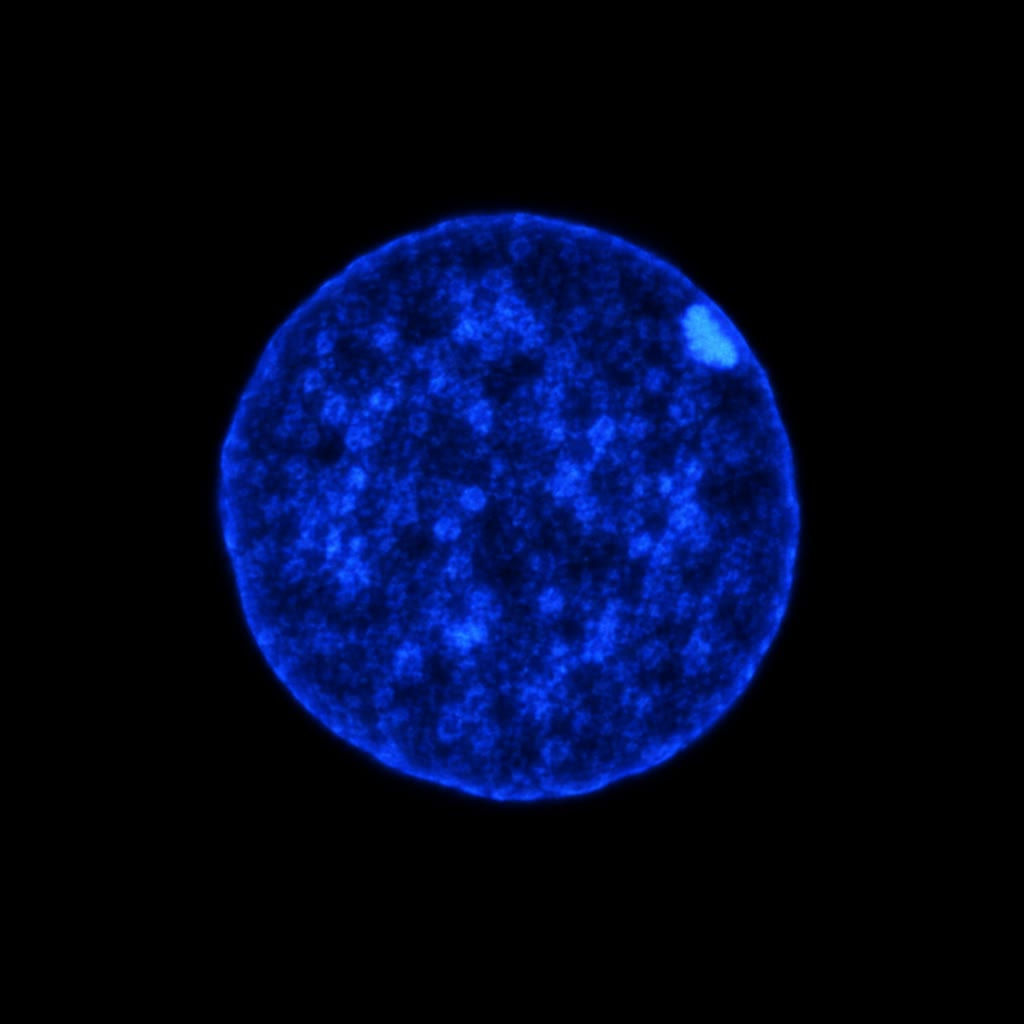
\includegraphics[width=0.42\linewidth]{images/book5/ai/b5-01-barr-body.jpg}\hspace{0.04\linewidth}
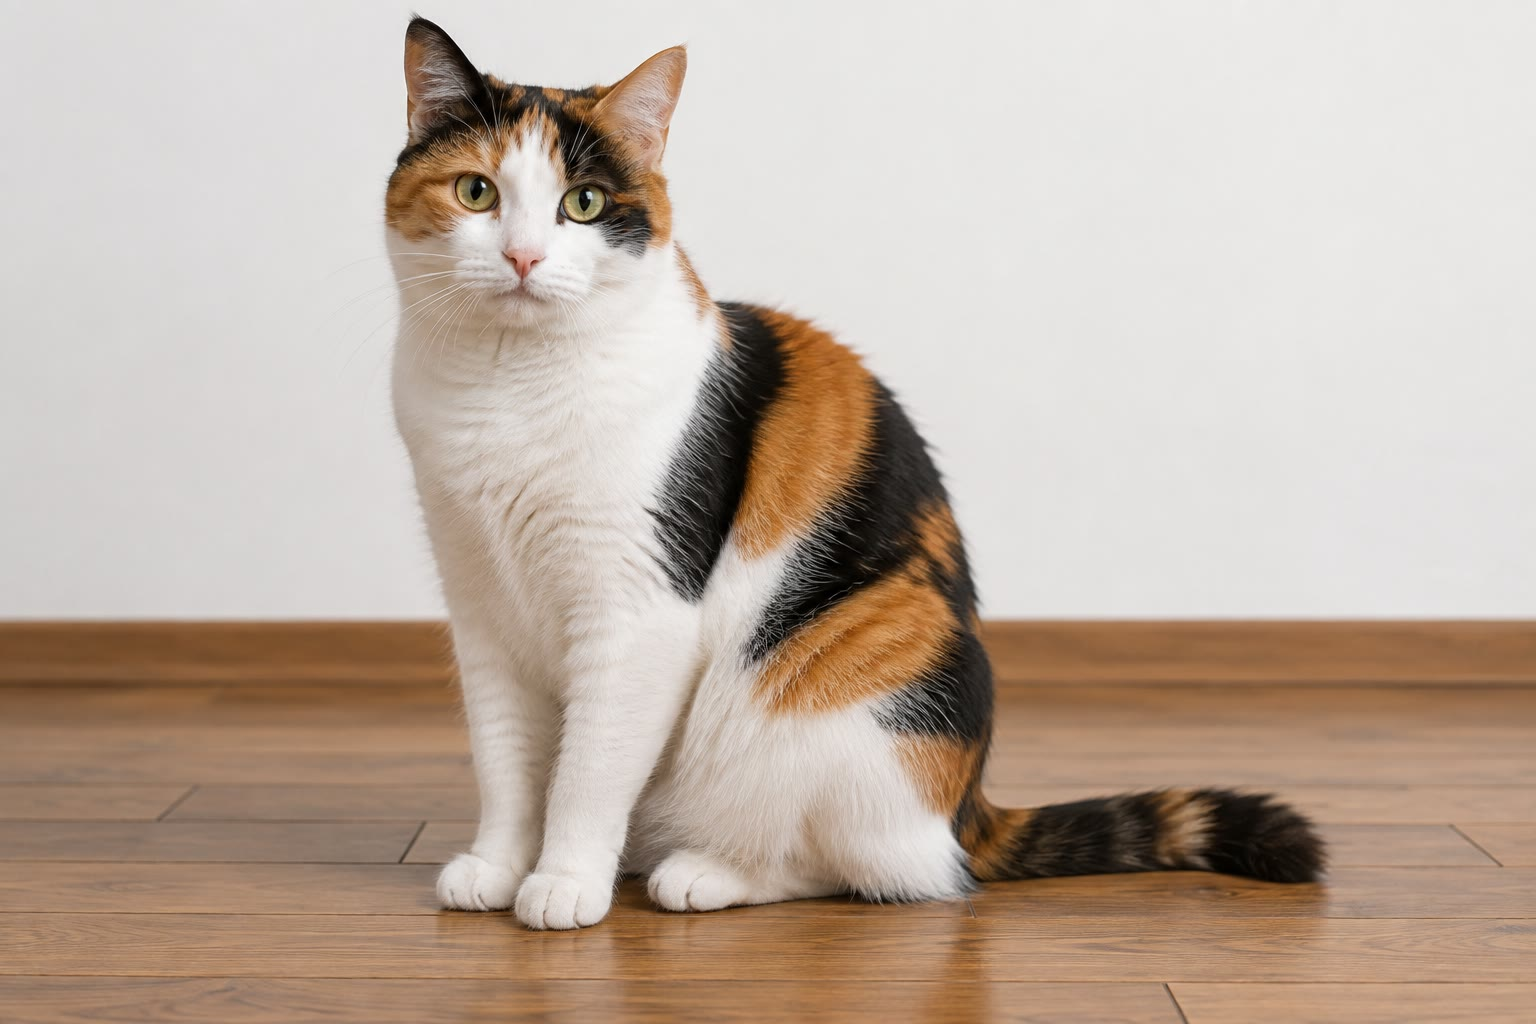
\includegraphics[width=0.5\linewidth]{images/book5/ai/b5-01-calico-cat.jpg}

{\small बाएँ: DNA के लिए अभिरंजित कोई मादा केंद्रक, जिसमें संघनित
निष्क्रिय X --- \omterm{def:b3:chromatin-epigenetics:x-inactivation}{बार पिंड} --- केंद्रक के किनारे से सटा है। दाएँ: कोई
कैलिको बिल्ली। हर नारंगी या काला धब्बा त्वचा-कोशिकाओं का ऐसा क्लोन है
जिसने वही X मौन किया; सफ़ेद रंग एक अलग, अलिंगसूत्री, धब्बा-जीन से आता
है।}
\end{omfigure}

\begin{definition}[जीनोमी अंकन]\label{def:b3:chromatin-epigenetics:imprinting}
\index{जीनोमी अंकन}\index{अंकन नियंत्रण क्षेत्र}\index{एकजनकीय द्विसूत्रता}
कोई जीन \emph{अंकित} तब है जब उसके दो युग्मविकल्पियों में से केवल एक
अभिव्यक्त होता है, और कौन-सा, यह इस पर निर्भर करता है कि वह किस जनक से
आया: कुछ जीन केवल पैतृक प्रति से अभिव्यक्त होते हैं, कुछ केवल मातृ
प्रति से। स्तनधारियों में लगभग \numrange{100}{200} अंकित जीन हैं, जो
गुच्छों में हैं, और हर गुच्छे पर किसी \emph{अंकन नियंत्रण क्षेत्र}
(ICR) का शासन है, जो एक जनकीय युग्मविकल्पी पर मेथिलित होता है और दूसरे
पर नहीं। मेथिलीकरण जनन-वंश में तय होता है --- शुक्राणु में एक प्रतिरूप,
अंडाणु में दूसरा ---, अगली पीढ़ी की जनन-कोशिकाओं में मिटा दिया जाता है
और उस व्यक्ति के लिंग के अनुसार फिर से तय किया जाता है। इसलिए जिस बच्चे
को किसी गुणसूत्र की दोनों प्रतियाँ एक ही जनक से मिलती हैं
(\emph{एकजनकीय द्विसूत्रता}) उसमें उस गुणसूत्र के अंकित जीनों की मात्रा
गलत होती है, यद्यपि उसका अनुक्रम पूरी तरह सामान्य है।
\end{definition}

\begin{proof}[प्रमाण-सामग्री]
मैकग्रा तथा सोल्टर ने, और स्वतंत्र रूप से सुरानी, बार्टन तथा नॉरिस
(1984) ने, निषेचित अंडाणुओं के बीच पूर्वकेंद्रक स्थानांतरित करके ऐसे
चूहा-युग्मनज बनाए जिनमें या तो दो मातृ पूर्वकेंद्रक थे या दो पैतृक।
इनमें से कोई भी पूर्ण अवधि तक विकसित नहीं हुआ, यद्यपि हर एक के पास
गुणसूत्रों के दो पूरे समुच्चय थे: स्त्रीजनित भ्रूणों ने ठीक-ठाक भ्रूण
बनाया पर अपरा दुर्बल रही, और पुंजनित भ्रूणों ने बड़ी अपरा बनाई और
भ्रूण लगभग कुछ नहीं। दोनों जनकीय जीनोम तुल्य नहीं हैं और दोनों
आवश्यक हैं। कैटानैच और कर्क (1985) ने गुणसूत्र-विशिष्ट एकजनकीय
द्विसूत्रताओं से दिखाया कि यह अतुल्यता विशेष गुणसूत्रों के विशेष
क्षेत्रों तक सीमित है, और वही वे क्षेत्र हैं जहाँ बाद में अंकित गुच्छे
मिले।
\end{proof}

\begin{example}[\emph{Igf2}--\emph{H19} गुच्छा]\label{ex:b3:chromatin-epigenetics:igf2}
\emph{Igf2}, एक भ्रूणीय वृद्धि कारक, पैतृक युग्मविकल्पी से अभिव्यक्त
होता है; उसका पड़ोसी \emph{H19}, एक अकूटलेखी RNA, मातृ से। उनके बीच
ICR है और, \emph{H19} से आगे, संवर्धकों का एक साझा समुच्चय। मातृ
गुणसूत्र पर ICR अमेथिलित होता है और CTCF से बँधता है, जो विद्युतरोधक
का काम करता है: संवर्धक \emph{H19} तक पहुँच सकते हैं पर \emph{Igf2}
तक नहीं। पैतृक गुणसूत्र पर ICR मेथिलित होता है (शुक्राणु में तय), CTCF
बँध नहीं सकता, और संवर्धक पार जाकर \emph{Igf2} तक पहुँच जाते हैं;
मेथिलीकरण फैलकर \emph{H19} प्रवर्तक को मौन भी कर देता है। एक ही चिह्न,
एक ही जनन-वंश में तय, दोनों जीनों का निर्णय करता है।
\end{example}

\begin{omfigure}
\begin{tikzpicture}[every node/.style={font=\scriptsize}, >=stealth]
  \foreach \yy/\lab/\ctcf in {1.6/मातृ गुणसूत्र/1, -0.6/पैतृक गुणसूत्र/0} {
    \draw[very thick, gray] (0,\yy) -- (9.4,\yy);
    \node[left, align=right] at (-0.15,\yy) {\lab};
    \draw[thick, fill=omDef!25] (1.0,\yy-0.2) rectangle (2.6,\yy+0.2); \node at (1.8,\yy) {\emph{Igf2}};
    \draw[thick, fill=omProp!30] (4.2,\yy-0.2) rectangle (5.2,\yy+0.2); \node at (4.7,\yy) {ICR};
    \draw[thick, fill=omDef!25] (6.2,\yy-0.2) rectangle (7.4,\yy+0.2); \node at (6.8,\yy) {\emph{H19}};
    \foreach \x in {8.4,8.8,9.2} \fill[omMeth!70!black] (\x,\yy) circle (0.12);
    \node[right] at (9.55,\yy) {संवर्धक};
  }
  % maternal: CTCF bound, enhancer -> H19
  \draw[thick, fill=omExo!35] (4.7,2.15) ellipse (0.45 and 0.22); \node at (4.7,2.15) {CTCF};
  \draw[->, thick, omMeth!70!black] (8.4,1.85) .. controls (7.8,2.5) and (7.2,2.5) .. (6.8,1.85);
  \node[above] at (7.6,2.35) {चालू};
  \draw[thick, omThm] (5.3,2.3) -- (5.3,0.9); \node[omThm, below] at (5.3,0.9) {विद्युतरोधक};
  \node[omThm, above=1.0cm, align=center, font=\scriptsize] at (1.8,1.8) {\emph{Igf2} मौन};
  % paternal: ICR methylated
  \foreach \x in {4.35,4.6,4.85,5.1} \fill[omThm] (\x,-0.95) circle (0.08);
  \node[below, align=center] at (4.7,-1.05) {मेथिलित:\\CTCF नहीं};
  \draw[->, thick, omMeth!70!black] (8.4,-0.35) .. controls (6.5,0.6) and (3.5,0.6) .. (1.8,-0.35);
  \node[above] at (3.3,0.2) {चालू};
  \foreach \x in {6.4,6.7,7.0,7.2} \fill[omThm] (\x,-0.95) circle (0.08);
  \node[below] at (6.8,-1.05) {मौन किया गया};
\end{tikzpicture}

{\small \emph{Igf2}--\emph{H19} पर अंकन। मातृ युग्मविकल्पी: अमेथिलित
ICR विद्युतरोधक CTCF से बँधता है, इसलिए नीचे के संवर्धक केवल
\emph{H19} को सक्रिय करते हैं। पैतृक युग्मविकल्पी: ICR शुक्राणु में
मेथिलित हुआ था, CTCF बँध नहीं सकता, संवर्धक \emph{Igf2} तक पहुँचते
हैं, और मेथिलीकरण \emph{H19} को मौन कर देता है।}
\end{omfigure}

\begin{example}[प्रैडर--विली और एंजेलमैन]\label{ex:b3:chromatin-epigenetics:pws}
गुणसूत्र 15 में लगभग \qty{5}{Mb} का वही विलोपन (क्षेत्र 15q11--q13)
\emph{प्रैडर--विली संलक्षण} --- जन्म पर दुर्बल पेशी-तान, फिर अतृप्त
भूख और मोटापा --- तब देता है जब वह पैतृक गुणसूत्र पर हो, और
\emph{एंजेलमैन संलक्षण} --- गंभीर बौद्धिक अक्षमता, वाणी का अभाव,
प्रसन्न मुद्रा और दौरे --- तब जब वह मातृ गुणसूत्र पर हो। इस क्षेत्र
में पैतृक रूप से अभिव्यक्त जीन हैं (\emph{SNRPN} और छोटे RNA का एक
गुच्छा), जिनकी एकमात्र सक्रिय प्रति पहली स्थिति में खो जाती है, और
मातृ रूप से अभिव्यक्त \emph{UBE3A}, जो दूसरी में खो जाता है। बिना किसी
विलोपन के भी, 15 की मातृ \omterm{def:b3:chromatin-epigenetics:imprinting}{एकजनकीय द्विसूत्रता} प्रैडर--विली देती है: दो
मातृ प्रतियाँ, पैतृक जीनों के लिए मौन।
\end{example}

\begin{remark}[अंकन क्यों]\label{rem:b3:chromatin-epigenetics:kinship}
अंकित जीनों में भ्रूणीय वृद्धि और अपरा के पोषक-हस्तांतरण के नियंत्रण
की बहुतायत है, जिनमें पैतृक रूप से अभिव्यक्त जीन (\emph{Igf2},
\emph{Peg3}) वृद्धि बढ़ाते हैं और मातृ रूप से अभिव्यक्त जीन
(\emph{H19}, \emph{Igf2r}, \emph{Cdkn1c}) उसे रोकते हैं। \emph{बंधुता
सिद्धांत} इसे एक द्वंद्व के रूप में पढ़ता है: पिता के जीनों को ऐसी
माता से अधिक खींच लेने में लाभ है जो आगे चलकर दूसरे नरों की संतति ढो
सकती है, जबकि माता के जीनों को अपने सारे प्रसवों में राशन बाँटने में
लाभ है। अंकन अपरा वाले स्तनधारियों में और सपुष्प पौधों में होता है,
जिनका भ्रूणपोष भी माता से पोषित होता है, और पक्षियों या सरीसृपों में
नहीं --- यही सिद्धांत की भविष्यवाणी है।
\end{remark}

\section{एपिजेनेटिक वंशागति और उसकी सीमाएँ}

\begin{definition}[एपिजेनेटिकी]\label{def:b3:chromatin-epigenetics:epigenetics}
\index{एपिजेनेटिकी}\index{एपियुग्मविकल्पी}\index{पुनःक्रमादेशन}
\emph{एपिजेनेटिकी} जीन-क्रियाशीलता के उन वंशागत परिवर्तनों का अध्ययन है
जो DNA अनुक्रम के परिवर्तन नहीं हैं: ऐसी अवस्थाएँ जो \omterm{def:b3:chromatin-epigenetics:methylation}{DNA मेथिलीकरण},
\omterm{def:b3:chromatin-epigenetics:nucleosome}{हिस्टोन} चिह्नों या स्वयं-पोषी अनुलेखन-कारक परिपथों से ढोई जाती हैं और
कोशिका-विभाजन के पार नकल होती हैं। समान अनुक्रम पर भिन्न स्थायी
एपिजेनेटिक अवस्था वाले दो युग्मविकल्पी \emph{एपियुग्मविकल्पी} हैं।
समसूत्री विभाजन के पार वंशागति नियम है और वही किसी विभेदित कोशिका को
विभेदित बनाए रखती है। अर्धसूत्री विभाजन के पार, जनक से संतति तक,
वंशागति स्तनधारियों में अपवाद है, क्योंकि चिह्न \emph{पुनःक्रमादेशन}
की दो लहरों में मिटा दिए जाते हैं: आद्य जनन-कोशिकाओं में, जहाँ अंकन और
अधिकांश मेथिलीकरण पोंछ दिए जाते हैं और फिर लिंग के अनुसार नए सिरे से
तय होते हैं, और दुबारा युग्मनज तथा प्रारंभिक भ्रूण में, जहाँ पैतृक
जीनोम TET3 द्वारा सक्रिय रूप से और मातृ जीनोम निष्क्रिय रूप से
अमेथिलित होता है, इससे पहले कि DNMT3 भ्रूण के अपने प्रतिरूप बिछाए।
\end{definition}

\begin{example}[अगूती जीवक्षम पीला चूहा]\label{ex:b3:chromatin-epigenetics:agouti}
$A^{vy}$ युग्मविकल्पी में \emph{अगूती} रोम-वर्ण जीन के ऊपर की ओर एक
रेट्रोट्रांसपोज़ॉन घुस गया है। जहाँ ट्रांसपोज़ॉन का प्रवर्तक अमेथिलित है वहाँ वह
हर कोशिका में \emph{अगूती} को लगातार चलाता है; चूहा पीला, मोटा और
मधुमेह-प्रवण होता है। जहाँ वह मेथिलित है वहाँ जीन अपने सामान्य
नियंत्रण में रहता है और चूहा भूरा होता है (``छद्म-अगूती'')। आनुवंशिक
रूप से समरूप सहोदर पूरे वर्णक्रम में फैले होते हैं, और किसी पीली माता
के पिल्ले किसी भूरी माता की तुलना में अधिक पीले होते हैं: मातृ जनन-वंश
से गुज़रते हुए \omterm{def:b3:chromatin-epigenetics:epigenetics}{एपियुग्मविकल्पी} अधूरा ही मिटता है। वॉटरलैंड और जर्टल
(2003) ने गर्भवती $A^{vy}$ माताओं को मेथिल-दाताओं (फ़ोलेट, विटामिन
B\textsubscript{12}, कोलीन, बीटेन) से समृद्ध आहार खिलाया और पिल्लों के
रोम भूरे की ओर खिसका दिए। एक पीढ़ी के परिवेश ने ऐसा चिह्न तय किया जिसे
अगली पीढ़ी ने ढोया।
\end{example}

\begin{omfigure}
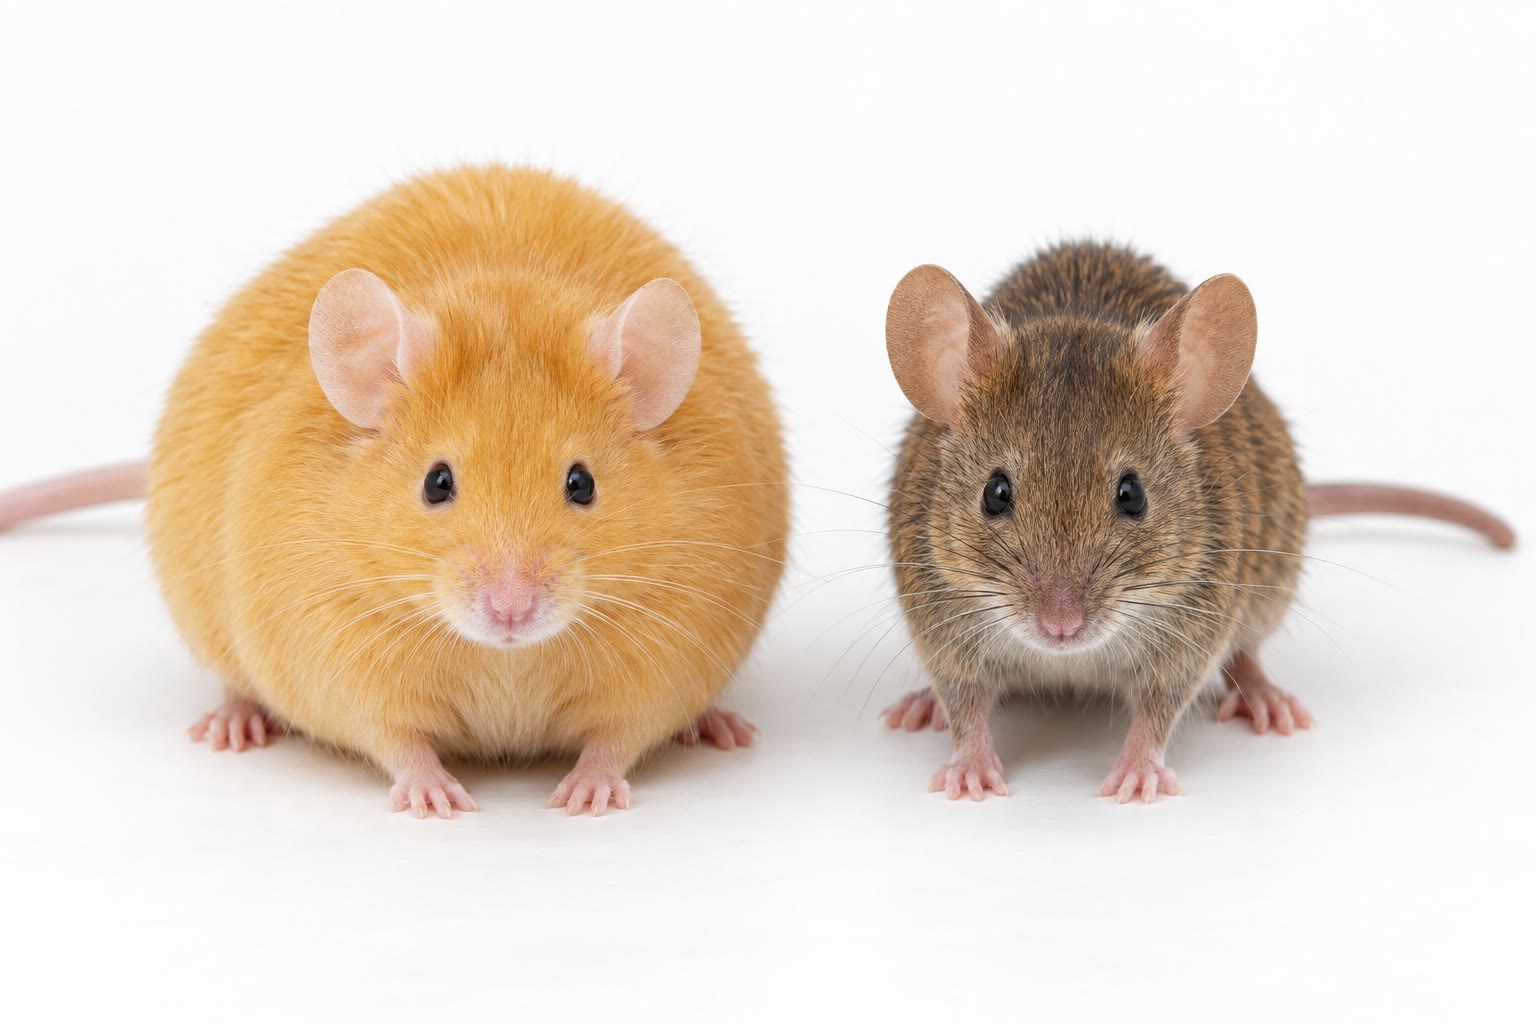
\includegraphics[width=0.62\linewidth]{images/book5/ai/b5-01-agouti-mice.jpg}

{\small समरूप जीन-प्ररूप वाले दो $A^{vy}$ सहोदर: एक पीला, मोटा चूहा
जिसमें \emph{अगूती} के ऊपर का ट्रांसपोज़ॉन अमेथिलित है, और एक भूरा
छद्म-अगूती जिसमें वह मेथिलित है।}
\end{omfigure}

\begin{proposition}[वंशागत एपिजेनेटिक अवस्थाएँ कहाँ मिलती हैं]\label{prop:b3:chromatin-epigenetics:examples}
\index{स्थिति-प्रभाव विचित्रवर्णता}\index{शीतीकरण}\index{परा-उत्परिवर्तन}
तीन भली-भाँति विश्लेषित तंत्र ऊपर की क्रियाविधियों को दर्शाते हैं।
\emph{Drosophila} में \emph{\omterm{prop:b3:chromatin-epigenetics:examples}{स्थिति-प्रभाव विचित्रवर्णता}}: किसी गुणसूत्र
पुनर्विन्यास से \omterm{def:b3:chromatin-epigenetics:nucleosome}{विषमक्रोमैटिन} के पास सरका दिया गया जीन कुछ कोशिकाओं में
मौन हो जाता है और कुछ में नहीं, जिससे चितकबरी आँख बनती है; हर धब्बा एक
क्लोन है, मौनीकरण HP1 पाश से \omterm{def:b3:chromatin-epigenetics:nucleosome}{विषमक्रोमैटिन} से फैलता है, और जिन जीनों का
उत्परिवर्तन विचित्रवर्णता को दबाता है (\emph{Su(var)} जीन) वे HP1 और
H3K9 मेथिलट्रांसफ़रेज़ हैं। \emph{Arabidopsis} में \emph{शीतीकरण}:
हफ़्तों की जाड़ी ठंड पुष्पन-दमनकारी \emph{FLC} को पॉलीकोम्ब-जमा
H3K27me3 से मौन कर देती है, यह मौनता वसंत की महीनों लंबी वृद्धि और
हज़ारों कोशिका-विभाजनों के पार बनी रहती है, और हर पीढ़ी में फिर से
शून्य कर दी जाती है, ताकि हर पौधे को अपनी जाड़ी स्वयं भोगनी पड़े। मक्के
में \emph{परा-उत्परिवर्तन}: \emph{b1} वर्णक जीन का एक युग्मविकल्पी, जब
किसी विषमयुग्मजी में एक विशेष दूसरे युग्मविकल्पी से मिलता है, उसे अपनी
ही मौन अवस्था में बदल देता है, और बदला हुआ युग्मविकल्पी वह अवस्था
पीढ़ियों तक अपने वंशजों को देता है, उस लघु-RNA-निर्देशित मेथिलीकरण से
जिसे \cref{ch:b3:rna-regulation} में उठाया गया है। हर स्थिति में
वंशागति समसूत्री और दृढ़ है; पीढ़ियों के पार संचरण या तो सक्रिय रूप से
शून्य कर दिया जाता है (पौधे) या रिसता और अधूरा होता है (चूहे)।
\end{proposition}

\begin{remark}[पीढ़ी-पार दावों की सीमाएँ]\label{rem:b3:chromatin-epigenetics:limits}
यह दावा कि किसी दादा-दादी का अकाल या तनाव मानव पोते-पोतियों को
``एपिजेनेटिक रूप से वंशागत'' हुआ है, आम है और अधिकतर अप्रमाणित। किसी
कायिक चिह्न और किसी पोते के बीच मिटाने की दो लहरें खड़ी हैं, स्तनधारियों
में अंकित जीन और थोड़े-से ट्रांसपोज़ॉन ही मिटाने के प्रलेखित उत्तरजीवी हैं, और
मानव समूहों में साझा परिवेश, गर्भाशयी परिवेश और आनुवंशिक भेदों के
प्रभावों को जनन-वंश में ढोए किसी चिह्न से अलग करना कठिन है। जो स्थितियाँ
सिद्ध हैं --- $A^{vy}$, कुछ ट्रांसपोज़ॉन-सहलग्न \omterm{def:b3:chromatin-epigenetics:epigenetics}{एपियुग्मविकल्पी}, कृमियों और
पौधों में RNA-मध्यस्थ अवस्थाएँ --- वे वास्तविक हैं, आणविक रूप से समझी
हुई हैं, और संकीर्ण हैं। अध्याय की प्रमेय बताती है क्यों: ऐसे पुनर्भरण
के बिना जो $\mu$ को $1$ तक धकेले, कोई चिह्न कुछ दर्जन विभाजनों में
स्वयं को भूल जाता है, और जनन-वंश उसके ऊपर एक सक्रिय शून्यीकरण जोड़ देता
है।
\end{remark}

\section{अभ्यास}

\begin{exercise}[$\star$]\label{exo:b3:chromatin-epigenetics:1}
\omterm{def:b3:chromatin-epigenetics:nucleosome}{न्यूक्लियोसोम} क्रोड-कण की संरचना, उससे बँधे DNA की लंबाई और प्रारूपिक
योजक-लंबाई दीजिए। \omterm{def:b3:chromatin-epigenetics:nucleosome}{क्रोमैटिन} के न्यूक्लिएज़-पाचन से धब्बे के बजाय खंडों
की सीढ़ी क्यों मिली?
\end{exercise}

\begin{exercise}[$\star$]\label{exo:b3:chromatin-epigenetics:2}
किसी मेढक के जीनोम में प्रति अगुणित समुच्चय $3.0\times 10^{9}$ क्षार
युग्म हैं। \qty{190}{bp} की पुनरावृत्ति मानकर किसी द्विगुणित केंद्रक
में कितने \omterm{def:b3:chromatin-epigenetics:nucleosome}{न्यूक्लियोसोम} होंगे, और उसका DNA कितना लंबा है?
\end{exercise}

\begin{exercise}[$\star$]\label{exo:b3:chromatin-epigenetics:3}
H3K27me3, H4K16ac और H3S10ph को खोलिए। हर एक के लिए बताइए कि वह सक्रिय
\omterm{def:b3:chromatin-epigenetics:nucleosome}{क्रोमैटिन} से जुड़ा है या मौन \omterm{def:b3:chromatin-epigenetics:nucleosome}{क्रोमैटिन} से, और पहले के लिए एक \omterm{def:b3:chromatin-epigenetics:histone-code}{पाठक} का
नाम दीजिए।
\end{exercise}

\begin{exercise}[$\star$]\label{exo:b3:chromatin-epigenetics:4}
समझाइए कि कोई कैलिको बिल्ली लगभग सदा मादा क्यों होती है, और कोई नर
कैलिको क्या होना चाहिए।
\end{exercise}

\begin{exercise}[$\star\star$]\label{exo:b3:chromatin-epigenetics:5}
\cref{def:b3:chromatin-epigenetics:nucleosome} के आँकड़ों से
(\qty{200}{bp} पुनरावृत्ति, \qty{11}{nm} मनका) \qty{10}{nm} तंतु का
\omterm{prop:b3:chromatin-epigenetics:compaction}{संवेष्टन अनुपात} निकालिए, और वह अनुपात भी जो किसी औसत मानव गुणसूत्र के
\qty{4}{cm} DNA को \qty{4}{\micro m} लंबे समसूत्री क्रोमैटिड में समाने
के लिए चाहिए। तंतु को और किस गुणक से मोड़ना पड़ेगा?
\end{exercise}

\begin{exercise}[$\star\star$]\label{exo:b3:chromatin-epigenetics:6}
\cref{thm:b3:chromatin-epigenetics:maintenance} के प्रतिरूप में
$\mu = 0.98$ और $\delta = 0.01$ लेकर $p^{*}$ निकालिए, और यह भी कि कितने
विभाजनों के बाद मेथिलित अवस्था से चला कोई स्थल $p^{*}$ पर अपने आधिक्य
का आधा खो देता है। $\mu = 0.999$, $\delta = 0.001$ के लिए दोहराइए।
\end{exercise}

\begin{exercise}[$\star\star$]\label{exo:b3:chromatin-epigenetics:7}
यकृत-कोशिकाओं पर किसी ChIP-seq प्रयोग में जीन $A$ के प्रवर्तक पर एक
H3K4me3 शिखर और एक H3K27ac शिखर मिलता है, जीन $B$ पर एक चौड़ा H3K27me3
प्रांत, और जीन $C$ पर H3K9me3। हर एक की अनुलेखन-अवस्था का पूर्वानुमान
कीजिए, और बताइए कि $B$ और $C$ में से किसके किसी दूसरे कोशिका-प्रकार में
चालू होने की अधिक संभावना है और क्यों।
\end{exercise}

\begin{exercise}[$\star\star$]\label{exo:b3:chromatin-epigenetics:8}
किसी स्त्री के एक गुणसूत्र 15 पर \emph{UBE3A} क्षेत्र का विलोपन है, फिर
भी वह स्वस्थ है। उसके पिता में भी वही विलोपन था और वे भी स्वस्थ थे।
उसके हर बच्चे को किस संलक्षण का, और कितनी प्रायिकता से, जोखिम है? यदि
विलोपन उसकी माता से आया होता तो?
\end{exercise}

\begin{exercise}[$\star\star$]\label{exo:b3:chromatin-epigenetics:9}
किसी मादा चूहा-भ्रूण में एक X गुणसूत्र से \emph{\omterm{def:b3:chromatin-epigenetics:x-inactivation}{Xist}} जीन हटाने के, और
दोनों से हटाने के, परिणाम का पूर्वानुमान कीजिए। किसी अलिंगसूत्र में
प्रविष्ट कराया गया \emph{\omterm{def:b3:chromatin-epigenetics:x-inactivation}{Xist}} पारजीन उस अलिंगसूत्र के साथ क्या करता
है, यह भी बताइए।
\end{exercise}

\begin{exercise}[$\star\star\star$]\label{exo:b3:chromatin-epigenetics:10}
\cref{ex:b3:chromatin-epigenetics:cpg-deficit} की सहायता से समझाइए कि
\omterm{def:b3:chromatin-epigenetics:methylation}{CpG द्वीपों} ने अपने \omterm{def:b3:chromatin-epigenetics:methylation}{CpG} क्यों बचाए रखे जबकि शेष जीनोम उनका
चार-पंचमांश खो चुका है, और इससे जनन-वंश में द्वीपों की
मेथिलीकरण-अवस्था के बारे में विकासात्मक काल-मान पर क्या निष्कर्ष
निकलता है। केवल यकृत में मेथिलित किसी जीन के लिए यह तर्क क्यों विफल
हो जाता है?
\end{exercise}

\begin{exercise}[$\star\star\star$]\label{exo:b3:chromatin-epigenetics:11}
\cref{prop:b3:chromatin-epigenetics:readers} के लेखक--पाठक पाश का
उपयोग करते हुए दिखाइए कि H3K9me3 का कोई प्रांत प्रतिकृति के पार स्थायी
कैसे रह सकता है, जबकि हर विभाजन चिह्नित \omterm{def:b3:chromatin-epigenetics:nucleosome}{हिस्टोनों} को नए अचिह्नित
\omterm{def:b3:chromatin-epigenetics:nucleosome}{हिस्टोनों} से दोगुना तनु कर देता है। प्रांत का फैलना कहाँ रुकेगा, यह
क्या तय करता है? अपने विवरण की जाँच के लिए कोई प्रयोग सुझाइए।
\end{exercise}

\begin{exercise}[$\star\star\star$]\label{exo:b3:chromatin-epigenetics:12}
कोई अध्ययन बताता है कि किसी अकाल से गुज़रे लोगों के पोते-पोतियों में
किसी वृद्धि-जीन पर मेथिलीकरण बदला हुआ है और शरीर-द्रव्यमान अधिक है। यह
निष्कर्ष निकालने से पहले कि कोई मेथिलीकरण-चिह्न जनन-वंश से संचरित हुआ,
किन वैकल्पिक व्याख्याओं को हटाना आवश्यक है, उन्हें गिनाइए, और बताइए कि
चूहों में कौन-सा प्रयोग प्रश्न का निपटारा कर देगा।
\end{exercise}

\section{समस्या: किसी मौन किए गए जीन की स्मृति}

\begin{problem}[{सप्तांत समस्या --- किसी मानव जीनोम को उसके केंद्रक में
ठूँसना, विभाजनों के पार किसी मेथिलीकरण-चिह्न का पीछा, किसी कैलिको
बिल्ली को क्लोनी मानचित्र की तरह पढ़ना, और किसी अंकित क्षेत्र के रोगों
की गिनती, जिसका अंत इस पर होता है कि बिना पुनर्भरण कोई चिह्न कितने
विभाजन जीता है और उस कोशिका-समष्टि का आकार क्या था जिसने अपना X चुना}]
\label{pb:b3:chromatin-epigenetics:1}
आँकड़े: किसी मानव द्विगुणित केंद्रक में $6.4\times 10^{9}$ क्षार युग्म
हैं, प्रति युग्म \qty{0.34}{nm} और \qty{650}{Da}; \omterm{def:b3:chromatin-epigenetics:nucleosome}{न्यूक्लियोसोम}
पुनरावृत्ति \qty{200}{bp} है, किसी \omterm{def:b3:chromatin-epigenetics:nucleosome}{हिस्टोन} अष्टलक का भार
\qty{108}{kDa} है, और कोई क्रोड-कण \qty{11}{nm} चौड़ी तथा \qty{5.5}{nm}
मोटी चकती है। केंद्रक \qty{10}{\micro m} व्यास का गोला है। जीनोम
\qty{42}{\%} G$+$C है। किसी सामान्य \omterm{def:b3:chromatin-epigenetics:methylation}{CpG} पर मेथिलीकरण: प्रति विभाजन
$\mu = 0.99$, $\delta = 0.02$।

\medskip
\noindent\textbf{भाग I --- संवेष्टन।}
\begin{enumerate}
  \item केंद्रक में DNA की कुल लंबाई और \omterm{def:b3:chromatin-epigenetics:nucleosome}{न्यूक्लियोसोमों} की संख्या
        निकालिए।
  \item \omterm{def:b3:chromatin-epigenetics:nucleosome}{हिस्टोन} (केवल अष्टलक) और DNA का कुल द्रव्यमान पिकोग्राम में
        निकालिए ($\qty{1}{Da} = \qty{1.66e-24}{g}$)।
  \item केंद्रक का आयतन और, क्रोड-कणों को बेलन मानकर, उनका कुल आयतन
        निकालिए। वे केंद्रक का कितना अंश भरते हैं?
  \item यदि \omterm{def:b3:chromatin-epigenetics:nucleosome}{न्यूक्लियोसोमों} को \qty{10}{nm} तंतु के रूप में सिरे से
        सिरा मिलाकर रखा जाए तो तंतु कितना लंबा होगा, और नग्न DNA की
        तुलना में \omterm{prop:b3:chromatin-epigenetics:compaction}{संवेष्टन अनुपात} क्या है?
  \item तंतु कोहेसिन से लंगर डाले \qty{200}{kb} के पाशों में मुड़ा है।
        कितने पाश, और प्रति पाश कितने \omterm{def:b3:chromatin-epigenetics:nucleosome}{न्यूक्लियोसोम}?
  \item स्वतंत्रता की मान्यता पर द्विगुणित जीनोम में कितने \omterm{def:b3:chromatin-epigenetics:methylation}{CpG}
        द्विन्यूक्लियोटाइड होते? प्रेक्षित संख्या $5.6\times 10^{7}$
        है। कितना अंश खो चुका है, और किस उत्परिवर्तनी क्रियाविधि से?
\end{enumerate}

\medskip
\noindent\textbf{भाग II --- विभाजनों के पार एक चिह्न।}
\begin{enumerate}[resume]
  \item $p_{n}$ के लिए पुनरावृत्ति-संबंध लिखिए और $p^{*}$ निकालिए।
  \item कोई प्रवर्तक \omterm{def:b3:chromatin-epigenetics:methylation}{CpG} $n = 0$ पर पूरी तरह मेथिलित है। $p_{n}$ का
        मान $10$, $50$ और $200$ विभाजनों के बाद निकालिए।
  \item कितने विभाजनों के बाद आधिक्य $p_{n} - p^{*}$ आधा हो जाता है?
        कोई ऊतक स्तंभ कोशिका लगभग सप्ताह में एक बार विभाजित होती है:
        यह कितने वर्ष हुए?
  \item कोई औषध \omterm{def:b3:chromatin-epigenetics:methylation}{DNMT1} को पूरी तरह रोक देती है ($\mu = 0$) और DNMT3 को
        भी ($\delta = 0$)। दिखाइए कि समष्टि में मेथिलित लड़ियों का अंश
        हर विभाजन पर आधा हो जाता है, और \qty{80}{\%} मेथिलीकरण को
        \qty{5}{\%} से नीचे लाने के लिए विभाजनों की संख्या निकालिए।
  \item किसी मौन किए गए द्वीप में मेथिल-CpG \omterm{def:b3:chromatin-epigenetics:histone-code}{पाठक} H3K9 मेथिलीकरण को
        बुलाते हैं, जो DNMT3 को बुलाता है, जिससे द्वीप के भीतर
        $\mu = 0.9995$ और $\delta = 0.0005$ हो जाता है। आधिक्य का
        अर्ध-आयु काल फिर से निकालिए, विभाजनों में और सप्ताह में एक
        विभाजन की दर से वर्षों में।
  \item एक वाक्य में समझाइए कि जीवन भर मौन रहने वाले किसी जीन को
        प्रश्न 11 का परिणाम क्यों चाहिए और प्रश्न 9 का क्यों नहीं, और
        किस प्रकार की आणविक व्यवस्था उसे पैदा करती है।
\end{enumerate}

\medskip
\noindent\textbf{भाग III --- कैलिको मानचित्र।}
\begin{enumerate}[resume]
  \item कोई बिल्ली X-सहलग्न नारंगी जीन के लिए विषमयुग्मजी है। समझाइए
        कि उसके रोम पर नारंगी और काले धब्बे क्यों हैं और एक धब्बा
        किसका प्रतिनिधित्व करता है।
  \item \omterm{def:b3:chromatin-epigenetics:x-inactivation}{X निष्क्रियण} तब हुआ जब त्वचा बनाने को नियत कोशिकाएँ $N$ थीं।
        हर एक ने यादृच्छिक रूप से एक X चुना। इसकी प्रायिकता क्या है कि
        सभी $N$ ने एक ही चुना, जिससे एकवर्णी बिल्ली बने?
  \item लगभग एक अरब बिल्लियों में ऐसी कोई एकवर्णी विषमयुग्मजी प्रलेखित
        नहीं है; प्रायिकता $10^{-9}$ लेकर $N$ का आकलन कीजिए।
  \item बिल्ली की त्वचा का पृष्ठ लगभग \qty{0.3}{m^2} है और उसके धब्बे
        औसतन \qty{15}{cm^2} के हैं। धब्बों की संख्या आँकिए, और समझाइए
        कि वह $N$ से बड़ी क्यों है।
  \item कोई XXY नर बिल्ला भी कैलिको है। उसकी कोशिकाओं में कितने \omterm{def:b3:chromatin-epigenetics:x-inactivation}{बार
        पिंड} दिखते हैं? किसी XXX मादा में और किसी XY नर में कितने?
  \item निष्क्रियण से बच निकलने वाला कोई जीन मादाओं में दो सक्रिय
        प्रतियों में और नरों में एक में होता है। ऐसा बचना सहनीय होने
        का एक कारण दीजिए और एक ऐसी स्थिति दीजिए जहाँ वह मायने रखता है।
\end{enumerate}

\medskip
\noindent\textbf{भाग IV --- गुणसूत्र 15।}
\begin{enumerate}[resume]
  \item प्रैडर--विली संलक्षण लगभग \num{15000} जन्मों में एक को होता
        है; \qty{70}{\%} स्थितियाँ पैतृक 15q11--q13 का नव विलोपन हैं
        और \qty{25}{\%} मातृ \omterm{def:b3:chromatin-epigenetics:imprinting}{एकजनकीय द्विसूत्रता}। हर कारण की जन्म-दर
        निकालिए।
  \item एंजेलमैन संलक्षण की बारंबारता लगभग उतनी ही है; \qty{70}{\%}
        मातृ विलोपन हैं, \qty{5}{\%} पैतृक द्विसूत्रताएँ और
        \qty{10}{\%} \emph{UBE3A} के बिंदु उत्परिवर्तन। बिंदु
        उत्परिवर्तन एंजेलमैन का कारण क्यों बनते हैं पर प्रैडर--विली का
        लगभग कभी नहीं?
  \item किसी पिता में ऐसा संतुलित स्थानांतरण है जो उसके \qty{20}{\%}
        शुक्राणुओं को 15q11--q13 का विलोपन देता है। उसके कितने अंश
        बच्चों को प्रैडर--विली होगा, और कितने अंश को एंजेलमैन?
  \item \omterm{def:b3:chromatin-epigenetics:imprinting}{एकजनकीय द्विसूत्रता} तब बनती है जब कोई त्रिसूत्री युग्मनज एक
        गुणसूत्र खो देता है। यदि कोई त्रिसूत्री-15 युग्मनज अपने तीन
        गुणसूत्रों में से एक यादृच्छिक रूप से खोए, और त्रिसूत्रता माता
        से आई हो (दो मातृ प्रतियाँ), तो उत्तरजीवी में मातृ
        द्विसूत्रता होने की प्रायिकता क्या है? कौन-सा संलक्षण?
  \item प्रैडर--विली के जीन पैतृक रूप से अभिव्यक्त हैं और एंजेलमैन का
        जीन मातृ रूप से। बंधुता सिद्धांत का उपयोग करके बताइए कि दोनों
        संलक्षणों के लक्षणों में से कौन-से (जन्म पर आहार-कठिनाई बनाम
        अतृप्त भूख) सिद्धांत से मेल खाते हैं और कौन-से मिलाना कठिन है।
  \item एंजेलमैन के उपचार के लिए मौन पैतृक \emph{UBE3A} को फिर से
        सक्रिय करने की एक विधि सुझाई गई है। उसकी मौनता किसी पैतृक रूप
        से अभिव्यक्त प्रतिसंवेदी RNA के कारण है। आणविक लक्ष्य सुझाइए
        और बताइए कि यह चिकित्सा दूसरे अंकित जीनों को क्यों नहीं
        छेड़ेगी।
  \item सारांश दीजिए: बिना पुनर्भरण (प्रश्न~9) और उसके साथ
        (प्रश्न~11) किसी चिह्न का अर्ध-आयु काल, विभाजनों में; और
        कैलिको रोम की संस्थापक समष्टि $N$ (प्रश्न~15)।
\end{enumerate}
\end{problem}
